\begin{frame}{Model}
\framesubtitle{General form}
    for u(x,t)
    \begin{equation}
    \text{ s.t. } u_t + \mathcal{N}[u] = 0
    \end{equation}
    def  
    \begin{equation}
    f := u_t + \mathcal{N}[u]
    \end{equation}
    Then the minimize problem is:
    \begin{equation}
    \min\limits_{u} MSE = MSE_u + MSE_f
    \end{equation}
    where
    \begin{equation}
    \text{MSE}_u = \frac{1}{N_u} \sum_{i=1}^{N_u} | u(t_i^u, x_i^u) - u_i |^2
    \end{equation}
    \begin{equation}
    \text{MSE}_f = \frac{1}{N_f} \sum_{i=1}^{N_f} | f(t_i^f, x_i^f) |^2
    \end{equation}
\end{frame}
\begin{frame}{Model}
    \begin{block}{Penalty term}
    When we refer to LASSO, the MSE term includes two part:\\
    the residual and the penalty (which is L^1 \text{norm of parameter})\\
    Now, it's actually setting the penalty term as:\\
    how far \( \mathscr{f} \)  is away from 0\\
    with the physics constrain: 
    \begin{equation}
    f := u_t + \mathcal{N}[u]=0
    \end{equation}
    \end{block}
\end{frame}

\begin{frame}{Model}
\framesubtitle{Discrete form and Runge-Kutta method}
    \begin{block}{Runge-Kutta method}
    (Example of a 4-step RK)
    Rewrite \( u_t + \mathcal{N}[u] = 0 \) in the form \( u_t = -\mathcal{N}[u] \).
    Start with \( u(0, x) = u_0(x) \):
    \begin{enumerate}
        \item Calculate the intermediate values \( k_1, k_2, k_3, k_4 \):
        \begin{align*}
            k_1 &= -\tau \mathcal{N}[u_n], \\
            k_2 &= -\tau \mathcal{N} \left( u_n + \frac{1}{2} k_1 \right), \\
            k_3 &= -\tau \mathcal{N} \left( u_n + \frac{1}{2} k_2 \right), \\
            k_4 &= -\tau \mathcal{N} \left( u_n + k_3 \right).
        \end{align*}

        \item Update the solution \( u \) at the next time step:
        \[
        u_{n+1} = u_n + \frac{1}{6} (k_1 + 2k_2 + 2k_3 + k_4).
        \]
    \end{enumerate}
    \end{block}
\end{frame}

\begin{frame}{Model}
\framesubtitle{Discrete form and Runge-Kutta method}
    Apply the q-step Runge-Kutta to the general form to create the discrete estimator:
    \begin{equation}
    u_{n+c_i} = u_n - \tau \sum_{j=1}^q a_{ij} N[u_{n+c_j}], \quad i = 1, \ldots, q
    \end{equation}
    \begin{equation}
    u_{n+1} = u_n - \tau \sum_{j=1}^q b_j N[u_{n+c_j}]
    \end{equation}
    And the SSE is:
    \begin{equation}
    \text{SSE}_n = \sum_{j=1}^{q+1} \sum_{i=1}^{N_n} \left| u_{n,j}(x_{n,i}) - u_{n,i} \right|^2
    \end{equation}
\end{frame}    


\begin{frame}{Model}
\framesubtitle{With boundary on function u (or multiple equations)}
    The solution of PDE could change large if the equation includes high order term.\\
    We may need to add boundary on u and add another penalty term to MSE function. That is:
    \begin{equation}
    \mathcal{B}(u) = 0
    \end{equation}
    \begin{equation}
    MSE = MSE_u + MSE_f + MSE_b
    \end{equation}
    where\\
    \( \methcal{B}[\text{ · }]\) is a boundary operator corresponding to Dirichlet, Neumann, Robin, or periodic boundary conditions. 
    \begin{equation}
    MSE_b = \frac{1}{N_b} \sum_{i=1}^{N_b} | \mathcal{B}(u)(t_i^b, x_i^b) |^2
    \end{equation}
    We could also apply the rule to any other u-equations.
\end{frame}
\begin{frame}{Model}
\framesubtitle{With weight on error}
    The error terms are not necessarily equally weighted.\\
    Given by Raissi, M., Perdikaris, P. , Karniadakis, G. E. (2024).
    An Expert’s Guide to Training Physics-informed Neural Networks.\\
    We could rewrite the MSE function as:
    \begin{equation}
    MSE = \lambda_u MSE_u + \lambda_f MSE_f + \lambda_b MSE_b
    \end{equation}
\end{frame}

\begin{frame}{Model}
\framesubtitle{With weight on error}
    and the \lambda s are estimated by:
    \begin{equation}
    \hat{\lambda}_u = \frac{\| \nabla_{\theta} \text{MSE}_u (\theta) \| + \| \nabla_{\theta} \text{MSE}_b (\theta) \| + \| \nabla_{\theta} \text{MSE}_f (\theta) \|}{\| \nabla_{\theta} \text{MSE}_u (\theta) \|}
    \end{equation}

    \begin{equation}
    \hat{\lambda}_f = \frac{\| \nabla_{\theta} \text{MSE}_f (\theta) \| + \| \nabla_{\theta} \text{MSE}_u (\theta) \| + \| \nabla_{\theta} \text{MSE}_b (\theta) \|}{\| \nabla_{\theta} \text{MSE}_f (\theta) \|}
    \end{equation}

    \begin{equation}
    \hat{\lambda}_b = \frac{\| \nabla_{\theta} \text{MSE}_b (\theta) \| + \| \nabla_{\theta} \text{MSE}_f (\theta) \| + \| \nabla_{\theta} \text{MSE}_u (\theta) \|}{\| \nabla_{\theta} \text{MSE}_b (\theta) \|}
    \end{equation}
    where \theta \text{ is} the parameter of network (weights and bias).
\end{frame}

\begin{frame}{Model}
\framesubtitle{Estimated result}
    In the Neural Network, we solve the minimize problem of MSE on all potential function u.\\
    There are two typical way of using the estimated result.
    \begin{enumerate}
        \item When we do not need the formula of u:\\
        Some times we only need the point estimate of the function. It could either because the analytical solution is hard to be solved in simple form, or because the point estimate is enough.
        
        \item When we need the formula of u:
        We should follow the steps to solve for a analytical solution of u.\\
        \begin{enumerate}
            \item solve the PDE with function parameters remained\(u(\gamma)\).
            \item set appropriate activation function.
            \item fit the model to get the estimated \(\hat{u}\).
            \item estimated the function parameter \(\gamma\) with \(\hat{u}\).
        \end{enumerate}
    \end{enumerate}
\end{frame}

\begin{frame}{Model}
\framesubtitle{Prediction failed}
    There are some cases that the prediction may failed:
    \begin{enumerate}
    \item Local minimum.
    \item Convergence difficulty.
    \item Chaotic system.
    \item Physics constraint.   
    \end{enumerate}
    I will list examples for third and fourth problem.
\end{frame}

\begin{frame}{Model}
\framesubtitle{Chaotic system}
    The paper: Steger, S., Rohrhofer, F. M.,  Geiger, B. C. (2022). How PINNs cheat: Predicting chaotic motion of a double pendulum. OpenReview shows the predicted result of a double pendulum movement.
    From the graph we could see, for different given condition at \(t_0\), the result could be extremely well fitted or totally unreliable.
    \begin{figure}[H]
        \centering
        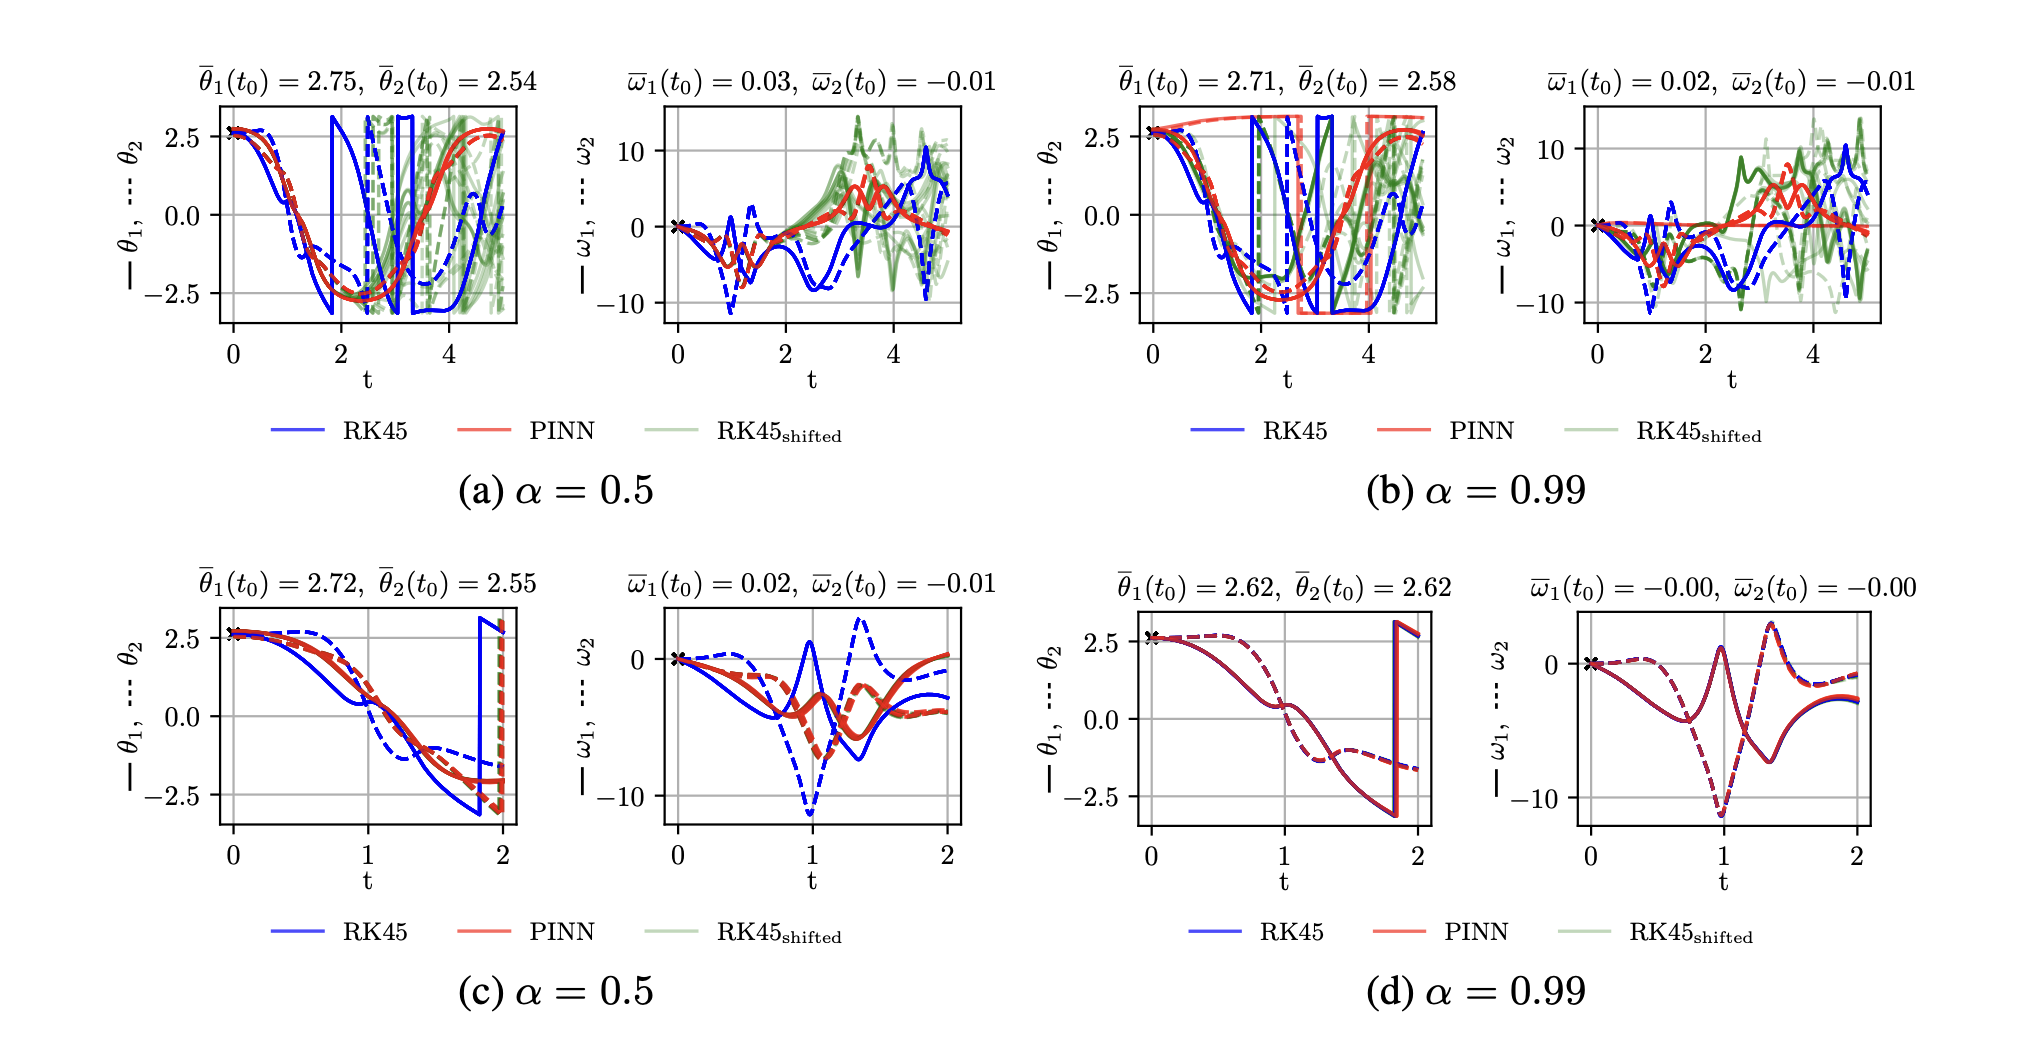
\includegraphics[width=0.8\textwidth]{img/Screenshot 2024-06-02 at 4.02.10 PM}
    \end{figure} 
\end{frame}

\begin{frame}{Model}
\framesubtitle{Violate physical causality}
    The paper: Wang, S., Yu, X.,  Perdikaris, P. (2022). Respecting causality is all you need for training physics-informed neural networks. \\

    In the paper, they discovered a convergence difficulty for the problem:
    \begin{equation}
    u_t - 0.0001u_{xx} + 5u^3 - 5u = 0, \quad t \in [0, 1], \quad x \in [-1, 1]
    \end{equation}
    \begin{equation}
    u(x, 0) = x^2 \cos(\pi x)
    \end{equation}
    \begin{equation}
    u(t, -1) = u(t, 1)
    \end{equation}
    \begin{equation}
    u_x(t, -1) = u_x(t, 1)
    \end{equation}
\end{frame}

\begin{frame}{Model}
\framesubtitle{Violate physical causality}
    They then find out that because the residual is fitted on each time spot that cannot capture the temporal causal relationships between physical variables. They adjust the loss function by adding a weight with causality parameter:
    \begin{equation}
    \mathcal{L}_r(\theta) = \frac{1}{N_t} \sum_{i=1}^{N_t} w_i \mathcal{L}_r(t_i, \theta)
    \end{equation}
    where
    \begin{equation}
    w_i = \exp \left( -\epsilon \sum_{k=1}^{i-1} \mathcal{L}_r(t_k, \theta) \right)
    \end{equation}
    and \(\epsilon\) is the causality parameter.
\end{frame}

\begin{frame}{Model}
\framesubtitle{Violate physical causality: fitting result}
    \begin{figure}[H]
        \centering
        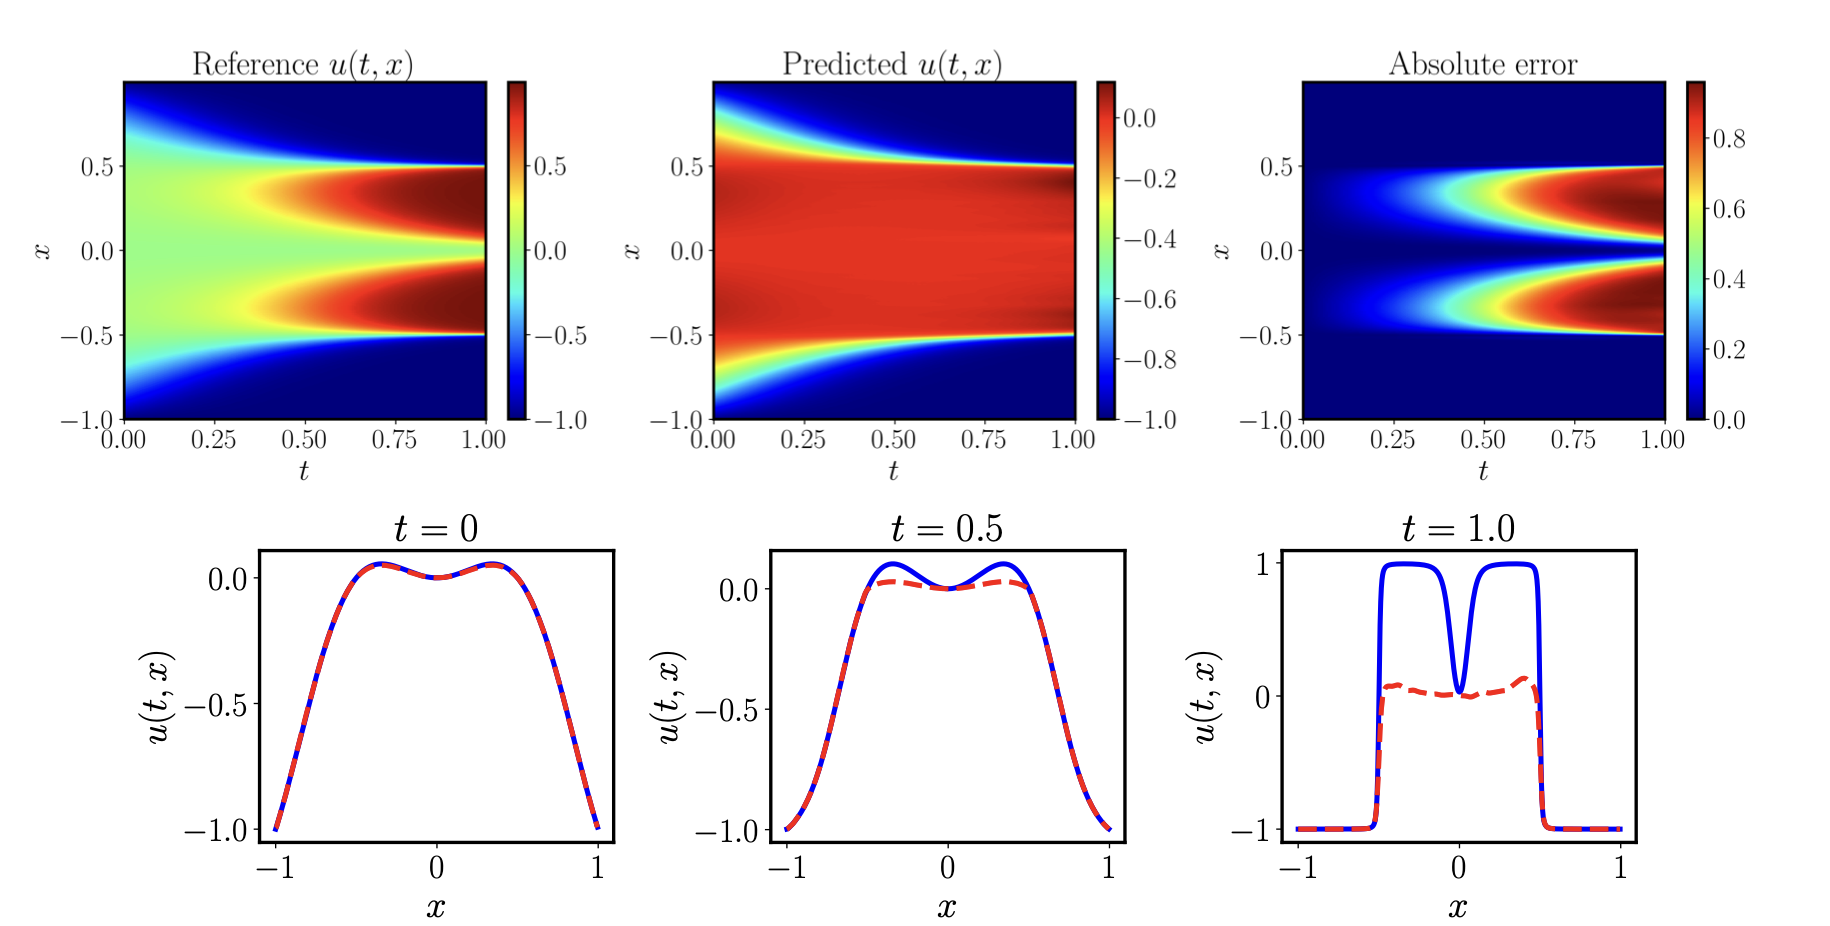
\includegraphics[width=0.55\textwidth]{img/Screenshot 2024-06-02 at 5.03.05 PM}
    \end{figure} 
    \begin{figure}[H]
        \centering
        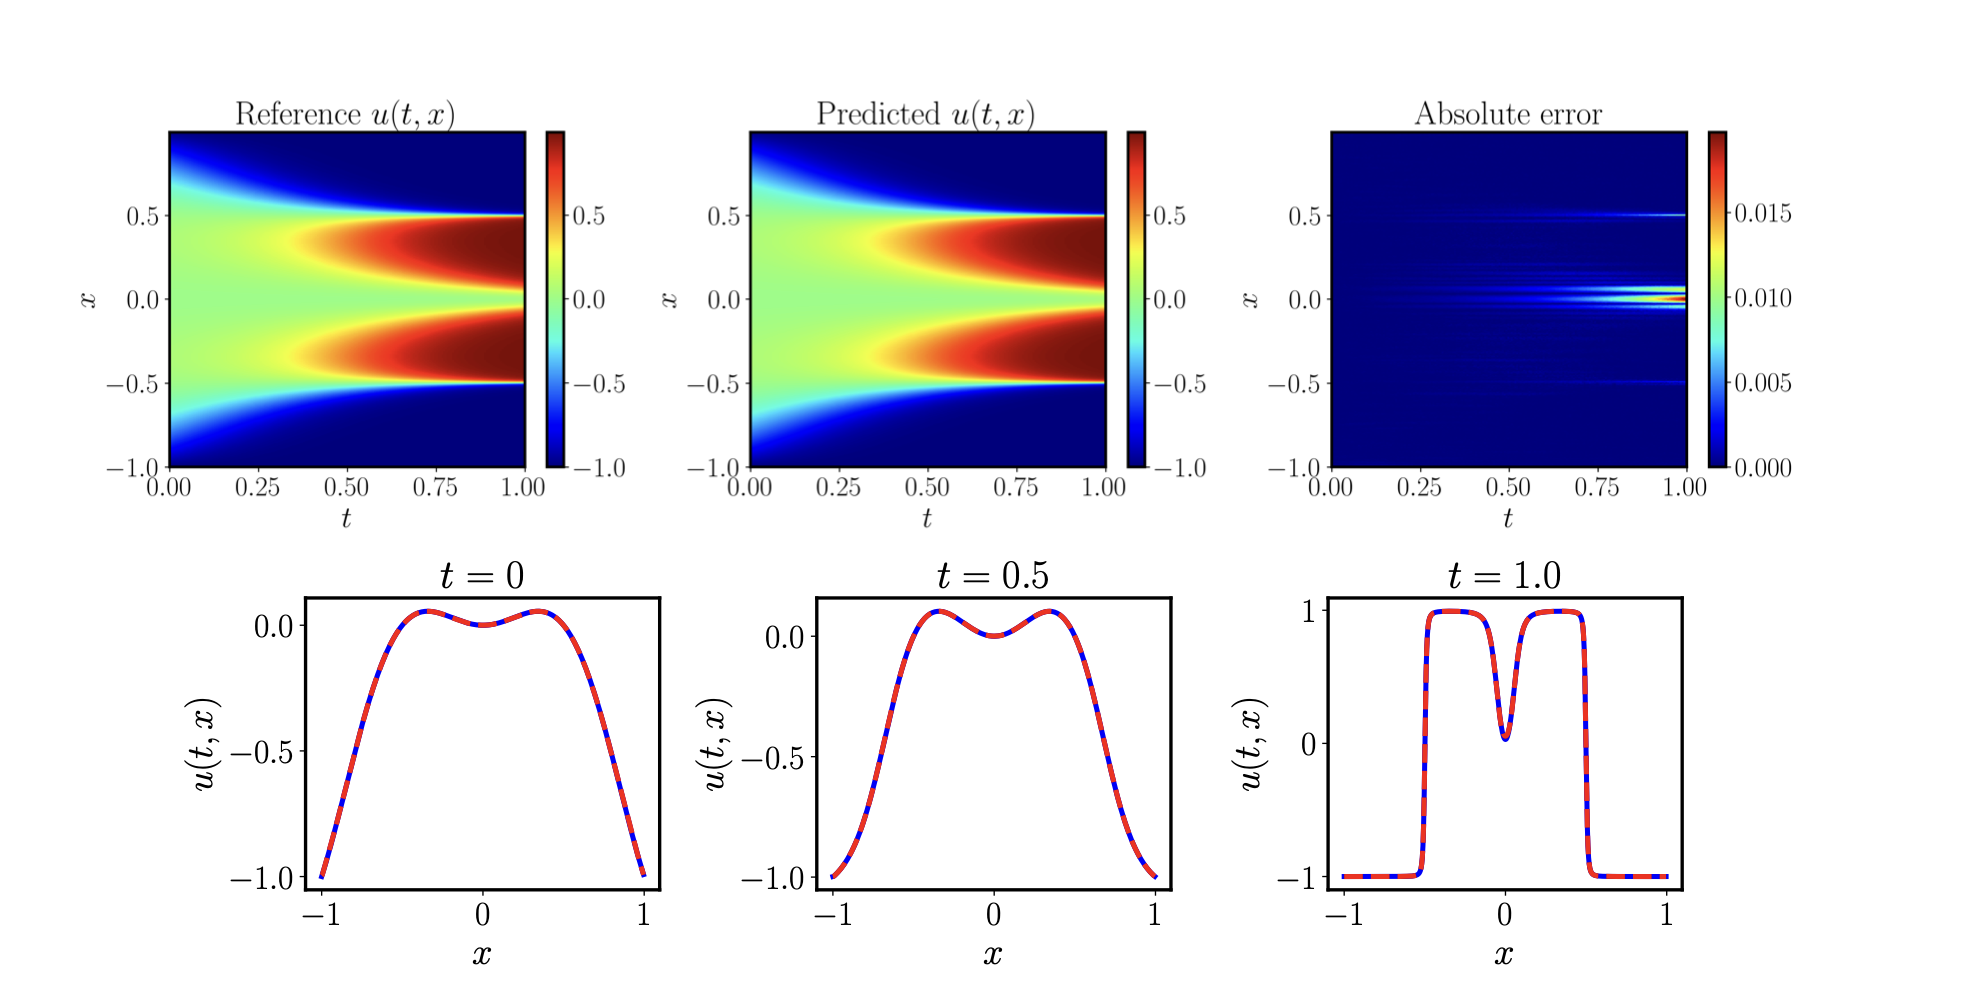
\includegraphics[width=0.6\textwidth]{img/Screenshot 2024-06-02 at 5.03.17 PM}
    \end{figure} 
\end{frame}